% Copyright 2026 Sreeram Anil
% SPDX-License-Identifier: CC-BY-4.0
\chapter{Embedded bootstrap particle filter (PF-Fast)}
\label{ch:pffast}

\section*{At a glance}
\begin{tabular}{@{}l>{\raggedright\arraybackslash}p{0.76\textwidth}@{}}
Family & Sequential Monte Carlo (particle / ensemble / Gaussian sum) \\
Header & \texttt{include/estkit/particle/pf\_fast.hpp} \\
Registered name & \texttt{PF-Fast} ($N=100$ particles) \\
State dimension & $n_x = 4$ (cell model) — generic in $n_x, n_u, n_y$ \\
Cost per step & \SI{16.0}{\micro\second}/step ($33\times$ EKF; $4.8\times$ faster than PF-Bootstrap) \\
Memory & \SI{9.7}{\kilo\byte} (one $N\times n_x$ state array; $4.8\times$ smaller) \\
Primary references & \cite{gordon1993,kitagawa1996,arulampalam2002,gustafsson2010pf,hol2006resampling} \\
\end{tabular}

\section{Motivation and aerospace/BMS relevance}
Chapter~\ref{ch:pfbootstrap} establishes that a particle filter can do things no Kalman filter can,
and that the textbook implementation costs \SI{76}{\micro\second} per cell per step and
\SI{46}{\kilo\byte} of RAM.  A 100-cell aviation battery sampled at \SI{10}{\hertz} would then need
\SI{76}{\milli\second} of CPU per second and \SI{4.6}{\mega\byte} of RAM --- both impossible on
the Cortex-M class parts that fly in a BMS slave board.  This chapter asks what the same algorithm
looks like when it is written for that target, and what it costs in accuracy.

Three things dominate the bill and all three are implementation, not mathematics:
\begin{enumerate}[label=(\roman*),leftmargin=2.5em]
  \item the number of particles $N$, which sets everything linearly;
  \item the \emph{second} $N\times n_x$ array that textbook resampling uses to hold the children
        while the parents are still being read;
  \item transcendental functions inside the per-particle loop --- a $\log$ or an $\exp$ costs
        \numrange{20}{40} cycles on an M7 against \numrange{1}{5} for a multiply-add.
\end{enumerate}
\estname{PF-Fast} removes (ii) entirely, reduces (iii) to a single $\exp$ per particle, and takes
$N = 100$.  The result is the same estimator as \estname{PF-Bootstrap} --- same proposal, same
weight recursion, same resampling distribution --- executed with one fifth of the samples, one
fifth of the memory and no auxiliary state buffer.

\section{Problem statement and assumptions}
Identical to Chapter~\ref{ch:pfbootstrap}: the model \eqref{eq:pfb-dyn}--\eqref{eq:pfb-meas}, the
ability to sample the transition density and to evaluate the likelihood.  The additional
requirements are of an engineering kind:
\begin{enumerate}[label=(B\arabic*),leftmargin=3em]
  \item bounded, statically known memory --- no heap, no recursion, no variable-length arrays;
  \item bounded, data-independent execution time --- the number of floating-point operations per
        step must not depend on the measurement values (it must be possible to certify a WCET);
  \item correct behaviour in \code{float32}, where the usable dynamic range of an exponential is
        $e^{-88}$ rather than $e^{-745}$.
\end{enumerate}
Requirement (B2) is the reason resampling is performed unconditionally in a fixed number of passes
rather than, say, by a loop that repeats until a target diversity is reached.

\section{Derivation}
The statistical content is the bootstrap recursion \eqref{eq:pfb-boot}; what follows is the
derivation of the three implementation choices.

\subsection{Weights in linear form with a single exponential}
The weight update $w^i \leftarrow w^i\, p(\vy_k\mid\vx_k^i)$ must be computed without overflow when
the log-likelihoods span hundreds of nats.  Write the Gaussian log-likelihood with the Cholesky
factor $\mR = \mL_R\mL_R^\T$ computed once per step:
\begin{equation}
  \ell^i = \log p(\vy_k\mid\vx_k^i)
         = \underbrace{-\sum_{m}\log (\mL_R)_{mm} - \tfrac{n_y}{2}\log 2\pi}_{c_0,\ \text{once per step}}
           \;-\; \tfrac12 \norm{\mL_R^{-1}\big(\vy_k - h(\vx_k^i,\vu_k)\big)}^2 .
  \label{eq:pff-loglik}
\end{equation}
The per-particle part of \eqref{eq:pff-loglik} is $n_y^2$ multiply-adds and \emph{no}
transcendental.  With $\ell_{\max} = \max_i \ell^i$ the update and normalisation are
\begin{equation}
  w^i \leftarrow w^i\, e^{\ell^i - \ell_{\max}}, \qquad
  w^i \leftarrow w^i \Big/ \sum_j w^j ,
  \label{eq:pff-wupdate}
\end{equation}
which is algebraically identical to $w^i \leftarrow w^i p(\vy_k\mid\vx_k^i)$ after normalisation
because the common factor $e^{\ell_{\max}}$ cancels.  Every exponent in \eqref{eq:pff-wupdate} is
in $(-\infty, 0]$, so the result is in $[0,1]$: it can only underflow to zero, never overflow, in
any precision.  Exactly one $\exp$ per particle is executed, and no $\log$ at all --- carrying the
weights in linear rather than logarithmic form is what removes the $\log$ that
Chapter~\ref{ch:pfbootstrap} needs to recentre its log-weights.

\subsection{In-place systematic resampling}
Systematic resampling \eqref{eq:pfb-systematic} is normally written as "compute parents $a(j)$,
then set $\vx^j_{\mathrm{new}} = \vx^{a(j)}_{\mathrm{old}}$", which needs the old array to survive
while the new one is written.  Express the same draw through the \emph{offspring counts}
\begin{equation}
  n^i = \#\{ j : a(j) = i \} = \#\Big\{ j : \textstyle\sum_{m<i} w^m \le \frac{j+u_0}{N} < \sum_{m\le i} w^m \Big\},
  \qquad \sum_i n^i = N,
  \label{eq:pff-counts}
\end{equation}
obtained in the same single pass over the cumulative weights.  Now observe:
\begin{itemize}[leftmargin=2em]
  \item a slot with $n^i = 0$ holds a particle that no child inherits --- its content is dead and
        may be overwritten immediately;
  \item a slot with $n^i = 1$ holds a particle with exactly one child, which may stay where it is
        --- \emph{no copy at all};
  \item a slot with $n^i > 1$ must push $n^i - 1$ copies of itself into dead slots.
\end{itemize}
Sweeping two cursors --- one looking for surplus parents, one looking for dead slots --- therefore
realises the resampled cloud in place.  Both cursors are monotone, so the sweep is $\mathcal{O}(N)$
and performs
$\sum_{i: n^i = 0} 1 = N - \#\{i : n^i > 0\}$
state copies, which is strictly fewer than the $2N$ copies of the textbook version and requires no
second state array.  Because systematic resampling keeps $n^i \in \{\lfloor Nw^i\rfloor, \lceil
Nw^i\rceil\}$, a cloud that has not yet degenerated moves almost nothing.

\begin{algorithm}[H]
\caption{In-place redistribution from offspring counts}
\begin{algorithmic}[1]
\Require particle array $\vx^{1:N}$, counts $n^{1:N}$ with $\sum_i n^i = N$
\State $s \gets 1$; \; $d \gets 1$
\Loop
  \While{$s \le N$ \textbf{and} $n^s \le 1$} \State $s \gets s+1$ \Comment{next parent with a surplus} \EndWhile
  \While{$d \le N$ \textbf{and} $n^d \ne 0$} \State $d \gets d+1$ \Comment{next dead slot} \EndWhile
  \If{$s > N$ \textbf{or} $d > N$} \State \textbf{break} \EndIf
  \State $\vx^d \gets \vx^s$; \quad $n^s \gets n^s - 1$; \quad $n^d \gets 1$
\EndLoop
\Ensure every slot holds a live particle, $n^i \equiv 1$
\end{algorithmic}
\end{algorithm}

\noindent The loop is safe because a slot is only ever written when $n^d = 0$, i.e.\ when nothing
still needs to read it; correctness does not depend on the ordering of $s$ and $d$
\cite[\S{}IV]{gustafsson2010pf}, \cite{hol2006resampling}.

\subsection{Roughening at small $N$}
The roughening scale \eqref{eq:pfb-roughen} contains $N^{-1/n_x}$, which for $n_x = 4$ grows from
\num{0.211} at $N=500$ to \num{0.316} at $N=100$: fewer samples are farther apart and need a wider
kernel to cover the gaps.  This is why $K$ is raised from \num{0.2} to \num{0.3} and the floor
$\varphi_{\min}$ from \num{0.005} to \num{0.01} of the prior standard deviation.  The cap
$\varphi_{\max} = 0.02$ is unchanged and remains essential
(Section~\ref{sec:pfb-battery}).

\section{Algorithm}
\begin{algorithm}[H]
\caption{PF-Fast --- one sampling period}
\begin{algorithmic}[1]
\Require particles $\{\vx_{k-1}^i\}$, linear weights $\{w_{k-1}^i\}$, $\vu_{k-1},\vu_k,\vy_k$
\State $\mL_Q \gets \operatorname{chol}(\mQ(\xhat_{k-1},\vu_{k-1}))$
\For{$i = 1$ \textbf{to} $N$} \Comment{time update, in place}
  \State $\vx_k^i \gets \operatorname{constrain}\big(f(\vx_{k-1}^i,\vu_{k-1}) + \mL_Q\bm{\xi}^i\big)$, \; $\bm{\xi}^i\sim\N{\bm 0}{\mI}$
\EndFor
\State $\yhat_k \gets \sum_i w_{k-1}^i h(\vx_k^i,\vu_k)$ \Comment{prior predictive}
\State $\mL_R \gets \operatorname{chol}(\mR)$; \; $c_0$ as in \eqref{eq:pff-loglik}
\For{$i = 1$ \textbf{to} $N$} \Comment{no transcendental here}
  \State $\ell^i \gets c_0 - \tfrac12\norm{\mL_R^{-1}(\vy_k - h(\vx_k^i,\vu_k))}^2$
\EndFor
\State $\ell_{\max} \gets \max_i \ell^i$
\For{$i = 1$ \textbf{to} $N$} \State $w^i \gets w_{k-1}^i \exp(\ell^i - \ell_{\max})$ \Comment{one $\exp$ per particle} \EndFor
\State $w^i \gets w^i / \sum_j w^j$; \quad $N_{\mathrm{eff}} \gets 1/\sum_i (w^i)^2$
\If{$N_{\mathrm{eff}} < \beta N$}
  \State counts $n^{1:N}$ from \eqref{eq:pff-counts} with one uniform; in-place redistribution; $w^i \gets 1/N$
  \State roughening \eqref{eq:pfb-roughen-clip} with $K = 0.3$, $\varphi_{\min}=0.01$, $\varphi_{\max}=0.02$
\EndIf
\State $\xhat_k \gets \sum_i w^i \vx_k^i$; \; $\mP_k \gets \sum_i w^i(\vx_k^i-\xhat_k)(\vx_k^i-\xhat_k)^\T$
\Ensure $\xhat_k$, $\mP_k$
\end{algorithmic}
\end{algorithm}

\section{Application to the battery model}
The filter sees the same cell model and the same likelihood \eqref{eq:pfb-celllik} as
Chapter~\ref{ch:pfbootstrap}; only $N$ and the roughening constants differ.  Two consequences are
specific to the cell:

\emph{The sampling cost is dominated by the model, not by the filter.}  One evaluation of $f$ for
the ESC model contains seven exponentials (two per Arrhenius-scheduled time constant, one for the
hysteresis factor) and one evaluation of $h$ contains one; the filter's own per-particle
arithmetic is four Gaussian draws and $n_y^2 = 1$ multiply-add.  Reducing $N$ is therefore the only
lever that matters, which is precisely why the algorithmic work went into making a small $N$ viable
(roughening) rather than into micro-optimising the weight loop.

\emph{The floor on the SOC jitter sets the recovery rate.}  With $\varphi_{\min} = 0.01$ and
$\sigma_{\soc_0} = 0.1$ the SOC jitter never falls below $10^{-3}$ per step.  The cloud can thus
walk about $3\times10^{-3}$ of SOC per step when the likelihood pulls consistently in one
direction, which is what produces the \SI{6.5}{\second} recovery from a \SI{35}{\percent}
initialisation error measured below.  At $N=100$ the best particle of the initial cloud sits at
about $2.5\sigma$ rather than the $3.1\sigma$ of $N=500$, which is why the transient peak error is
\SI{10.1}{\percent} here against \SI{5.0}{\percent} for \estname{PF-Bootstrap}: small clouds have
thin tails.

\section{Implementation notes}
\emph{Storage} (measured, \code{sizeof}): \SI{9.66}{\kilo\byte} against \SI{46.5}{\kilo\byte} for
\estname{PF-Bootstrap}, a factor \num{4.8}.  The breakdown at $N=100$, $n_x=4$, double precision:
\SI{3.2}{\kilo\byte} particles, \SI{0.8}{\kilo\byte} weights, \SI{0.8}{\kilo\byte} likelihoods,
\SI{0.4}{\kilo\byte} counts, \SI{4.3}{\kilo\byte} model copy (the OCV table dominates and is shared
in a real deployment).  In \code{float32} the particle array halves again.

\emph{Determinism.}  Every branch in the per-particle loops is loop control; the only
data-dependent branch in the step is the ESS test, and both of its outcomes have bounded cost.  The
resampling sweep executes at most $N$ copies.  The step is therefore WCET-analysable, which is a
certification requirement for anything that feeds a flight-critical energy estimate
\cite{rtca2017do311a}.

\emph{Float32.}  The single-precision build reproduces the double-precision result exactly to
within Monte-Carlo noise: $\mathrm{RMSE}_{\mathrm{ss}} = \SI{0.22}{\percent}$ in both precisions on
\code{nominal} (Table~\ref{tab:float}).  That is the point of \eqref{eq:pff-wupdate}.

\emph{Numerical range.}  \eqref{eq:pff-wupdate} never overflows.  Underflow to $w^i = 0$ is
harmless: such a particle is dead and will be replaced by the next resampling, and the
normalisation is guarded so that an all-zero weight vector resets the cloud to uniform instead of
producing NaNs.  This is the failure mode that makes a naive $\prod p(\vy\mid\vx)$ implementation
useless in \code{float32}, and it is the reason the log-domain likelihood
\eqref{eq:pff-loglik} is retained even though the weights themselves are linear.

\emph{Cost.}  Measured \SI{16.0}{\micro\second}/step (ECM \code{nominal}; range over the twelve
scenarios \SIrange{16.0}{18.9}{\micro\second}), against \SI{76.4}{\micro\second} for
\estname{PF-Bootstrap} --- a speed-up of \num{4.8}, i.e.\ essentially the particle ratio, confirming
that the removed buffer copy and the removed logarithms are second-order next to the model
evaluations, which scale exactly with $N$.  Against the EKF (\SI{477}{\nano\second}) the factor is
\num{33}.  The runtime table's projection to a Cortex-M7 class processor ($\kappa=30$,
Chapter~\ref{ch:metrics}) is \SI{480}{\micro\second} per cell per step: about \num{200} cells
per core at \SI{1}{\hertz}, or twenty at \SI{10}{\hertz}, which places \estname{PF-Fast} at the boundary of practicality for a
module-level (not pack-level) deployment.

\section{Benchmark results}
% Copyright 2026 Sreeram Anil
% SPDX-License-Identifier: CC-BY-4.0
\begin{table}[H]\centering\footnotesize\setlength{\tabcolsep}{4pt}
\caption{PF-Fast: cell-level benchmark on the eVTOL mission (mean over seeds; RMSE and max error in \% SOC; $t_\mathrm{conv}$: first time the error stays below 2\,\% for 60\,s, -- = never; EKF reference: steady-state RMSE of the plain EKF on the same data).}\label{tab:cell_PFFast}
\begin{tabular}{llrrrrrcrr}\toprule
plant & scenario & RMSE & RMSE$_\mathrm{ss}$ & max & $t_\mathrm{conv}$ [s] & RMSE$_v$ [mV] & div. & EKF ref. & ns/step \\ \midrule
ECM & nominal & 0.21 & 0.18 & 0.93 & 0 & 0.92 & no & 0.05 & 15960 \\
ECM & init\_error & 0.41 & 0.18 & 10.13 & 5 & 2.47 & no & 0.05 & 16018 \\
ECM & current\_bias & 0.99 & 0.91 & 3.25 & 0 & 0.94 & no & 0.61 & 15973 \\
ECM & noise\_step & 0.57 & 0.68 & 2.35 & 0 & 3.87 & no & 0.12 & 18898 \\
ECM & outliers & 0.39 & 0.39 & 1.66 & 0 & 1.52 & no & 0.21 & 16454 \\
ECM & cold & 0.62 & 0.57 & 2.19 & 0 & 1.97 & no & 0.16 & 15945 \\
ECM & hot & 0.19 & 0.14 & 0.96 & 0 & 0.71 & no & 0.03 & 16023 \\
ECM & aged\_cell & 3.43 & 2.62 & 15.14 & 0 & 4.04 & no & 1.52 & 16862 \\
ECM & param\_mismatch & 2.26 & 1.75 & 11.01 & 0 & 2.96 & no & 1.36 & 16369 \\
ECM & sensor\_dropout & 0.46 & 0.20 & 7.20 & 0 & 1.83 & no & 0.46 & 15990 \\
ECM & preisach & 1.45 & 1.00 & 5.03 & 148 & 0.95 & no & 0.20 & 16117 \\
ECM & combined & 3.25 & 2.52 & 16.70 & 1 & 5.47 & no & 12.44 & 16628 \\
\midrule
SPM & nominal & 1.14 & 0.91 & 3.74 & 144 & 1.05 & no & 3.73 & 15536 \\
SPM & init\_error & 1.39 & 0.89 & 10.13 & 246 & 2.32 & no & 3.81 & 15726 \\
SPM & current\_bias & 1.34 & 1.01 & 4.46 & 248 & 1.10 & no & 5.69 & 15649 \\
SPM & noise\_step & 1.17 & 0.94 & 3.74 & 144 & 3.93 & no & 3.30 & 18364 \\
SPM & outliers & 1.40 & 1.28 & 4.95 & 0 & 1.62 & no & 1.99 & 16052 \\
SPM & cold & 4.03 & 4.37 & 15.26 & 563 & 5.56 & no & 7.35 & 15805 \\
SPM & hot & 0.95 & 0.87 & 3.46 & 101 & 0.78 & no & 2.16 & 15553 \\
SPM & param\_mismatch & 2.84 & 1.78 & 10.44 & 180 & 1.89 & no & 3.13 & 15726 \\
SPM & sensor\_dropout & 1.32 & 1.05 & 8.20 & 129 & 2.09 & no & 5.31 & 15599 \\
\bottomrule\end{tabular}\end{table}

\begin{figure}[H]\centering
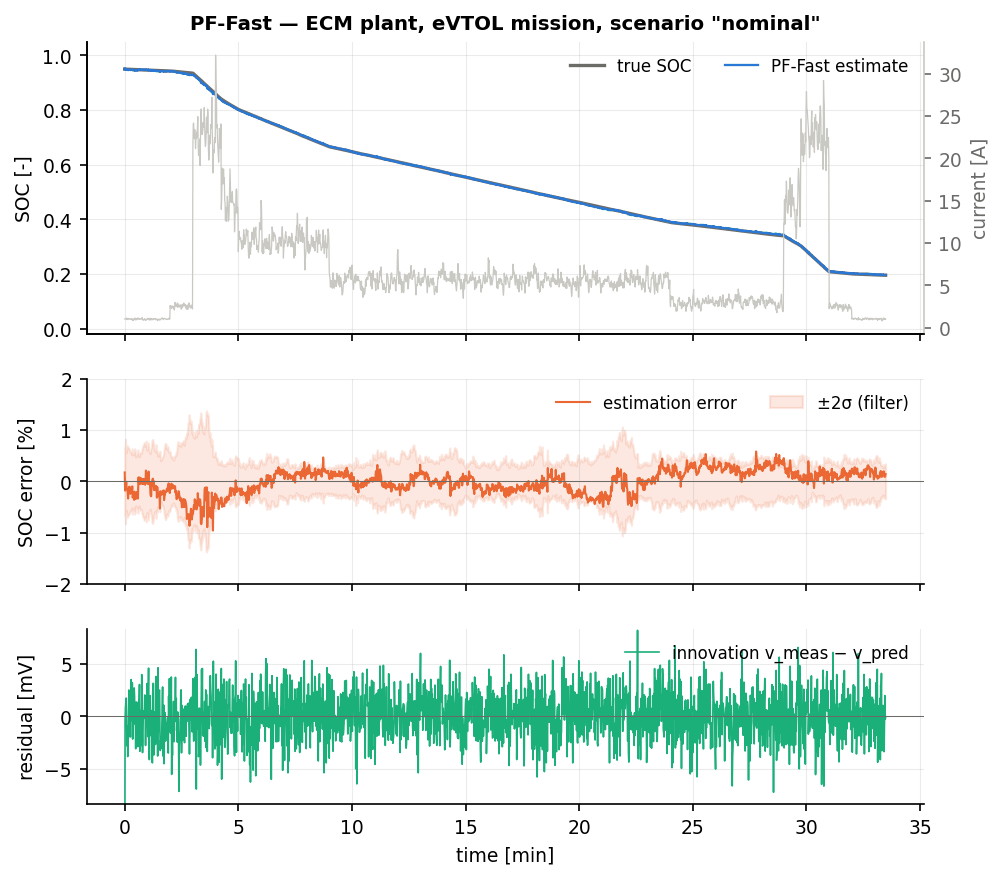
\includegraphics[width=\textwidth]{figures/cell_PFFast_nominal.png}
\caption{PF-Fast on the nominal eVTOL mission: true and estimated SOC (top), estimation error with
the $\pm2\sigma$ band from the weighted particle covariance (middle), voltage residual (bottom).}
\end{figure}
\begin{figure}[H]\centering
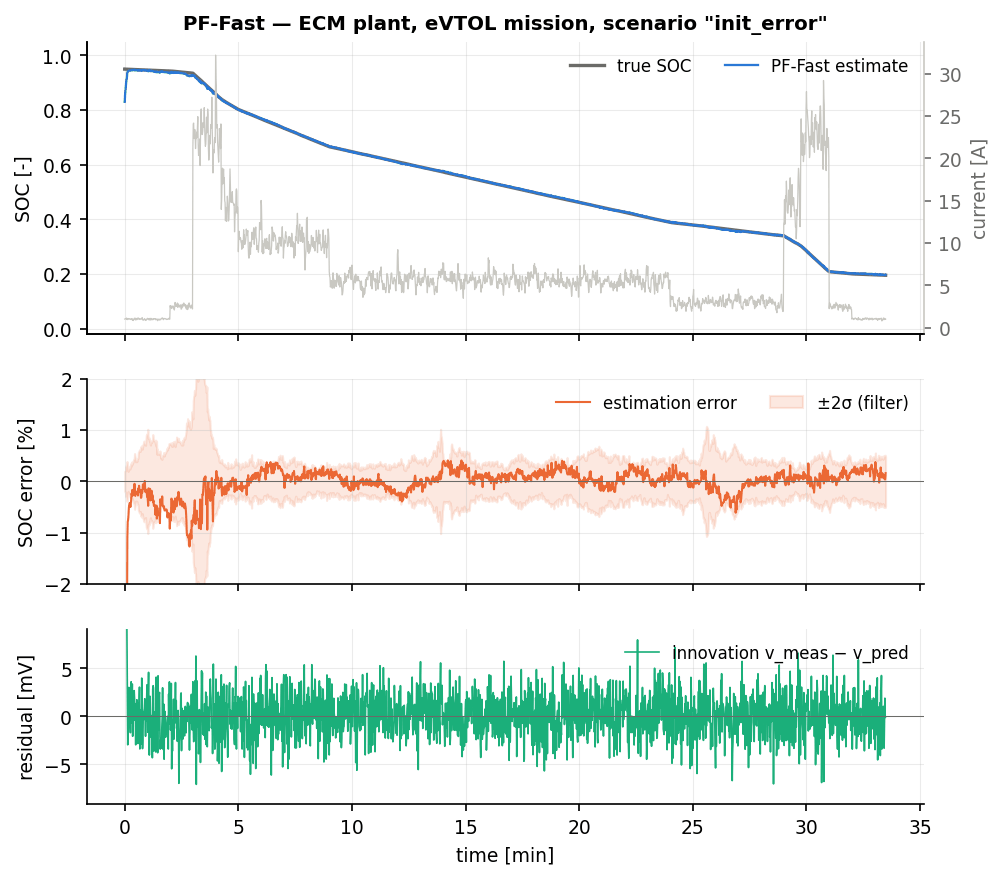
\includegraphics[width=\textwidth]{figures/cell_PFFast_init_error.png}
\caption{PF-Fast with a \SI{35}{\percent} initial SOC error: recovery within a few seconds, with a
larger transient peak than the $N=500$ filter (\SI{10.1}{\percent} against \SI{5.0}{\percent})
because a 100-particle cloud has thinner tails.}
\end{figure}
\begin{figure}[H]\centering
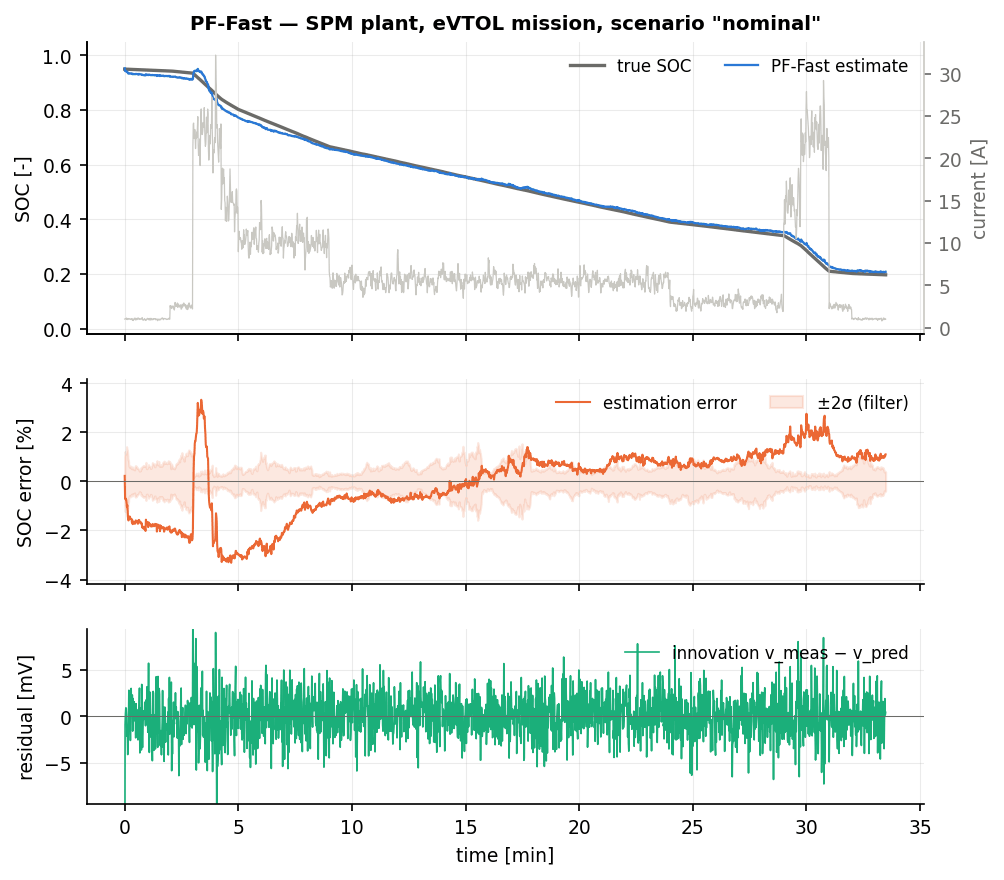
\includegraphics[width=\textwidth]{figures/cellspm_PFFast_nominal.png}
\caption{PF-Fast on the electrochemical (SPM) plant, nominal mission.  One hundred particles are
enough to keep the structured \SI{4}{\milli\volt} model residual out of the SOC estimate.}
\end{figure}

\paragraph{ECM plant.}  On \code{nominal} the filter achieves $\mathrm{RMSE} = \SI{0.21}{\percent}$,
$\mathrm{RMSE}_{\mathrm{ss}} = \SI{0.18}{\percent}$, maximum error \SI{0.93}{\percent}, immediate
convergence and a voltage-residual RMSE of \SI{0.92}{\milli\volt}.  Compared with
\estname{PF-Bootstrap} (\SI{0.16}{\percent} at \SI{76.4}{\micro\second}) the accuracy loss is a
factor of only \num{1.13} for a speed-up of \num{4.8} and a memory reduction of \num{4.8}.  The
naive $N^{-1/2}$ argument would predict $\sqrt{500/100} = \num{2.2}$; the observed \num{1.13} says
that at these sample sizes the estimator is not sampling-limited at all but limited by the
roughening floor, which both filters share.  Five-fold savings are therefore essentially free on
this problem, and that is the single most useful result of this chapter.

Across the scenario set: \code{init\_error} \SI{0.18}{\percent} with convergence in
\SI{5}{\second} (against \SI{73}{\second} for the 500-particle filter, whose slowest seed lingers
just above the \SI{2}{\percent} band --- at $N=100$ the wider roughening kernel actually crosses it
sooner), \code{outliers} \SI{0.39}{\percent} against \SI{0.36}{\percent}, \code{sensor\_dropout}
\SI{0.20}{\percent} against \SI{0.13}{\percent}, \code{param\_mismatch} \SI{1.75}{\percent} against
\SI{1.72}{\percent}, \code{aged\_cell} \SI{2.62}{\percent} against \SI{2.54}{\percent} and
\code{combined} \SI{2.52}{\percent} against \SI{2.76}{\percent} --- the small cloud is, if anything,
marginally better on the two hardest scenarios.  The largest relative penalties are
\code{noise\_step} (\SI{0.68}{\percent} against \SI{0.51}{\percent}), where a small cloud has less
redundancy to absorb a tenfold increase in measurement noise that the fixed $\mR$ does not know
about, and \code{cold} (\SI{0.57}{\percent} against \SI{0.33}{\percent}).  Divergence never occurs,
and the peak error over all twelve ECM scenarios is \SI{16.7}{\percent} (\code{combined}), against
\SI{15.2}{\percent} for the 500-particle filter.

\paragraph{SPM plant.}  On the electrochemical plant \estname{PF-Fast} gives
$\mathrm{RMSE}_{\mathrm{ss}} = \SI{0.91}{\percent}$ on \code{nominal} against \SI{3.73}{\percent}
for the EKF --- a factor of \num{4.1} --- and it is the weakest of the four full-state particle
filters there (\estname{PF-Auxiliary} \SI{0.62}{\percent}, \estname{PF-Regularized}
\SI{0.64}{\percent}, \estname{PF-Bootstrap} \SI{0.73}{\percent}).  This is the one place where the
sample size shows: the structured \SI{4}{\milli\volt} residual has to be spread over SOC and the
RC states, and with a hundred particles the cloud resolves that trade-off more coarsely, which also
costs it convergence time (\SI{144}{\second} on SPM \code{nominal} against \SI{0}{\second} for
$N=500$).  The mechanism is otherwise exactly the one described in Chapter~\ref{ch:pfbootstrap}:
the jitter keeps the slow RC state free to take up the persistent part of the residual, so the
model error appears in the voltage residual (\SI{1.05}{\milli\volt}) instead of in the SOC.  The
remaining SPM rows follow the same pattern --- \code{current\_bias} \SI{1.01}{\percent} (EKF
\SI{5.69}{\percent}), \code{param\_mismatch} \SI{1.78}{\percent} (EKF \SI{3.13}{\percent}),
\code{sensor\_dropout} \SI{1.05}{\percent} (EKF \SI{5.31}{\percent}), \code{cold}
\SI{4.37}{\percent} (EKF \SI{7.35}{\percent}) --- with no divergence anywhere.

\section{Summary}
\estname{PF-Fast} is the bootstrap filter written the way an embedded engineer would write it: one
state array, one exponential per particle, a resampling sweep with two monotone cursors and no
auxiliary storage, and a roughening kernel widened to suit a hundred samples.  It delivers
\SI{16.0}{\micro\second}/step and \SI{9.7}{\kilo\byte} --- factors of \num{4.8} on both counts
against the textbook implementation --- at the cost of only \num{1.13} in steady-state SOC RMSE on
the ECM plant (\SI{0.18}{\percent} instead of \SI{0.16}{\percent}) and about \num{1.25} on the SPM
plant (\SI{0.91}{\percent} instead of \SI{0.73}{\percent}, against \SI{3.73}{\percent} for the
EKF).  Single precision costs nothing measurable.  Use it when a particle filter is genuinely
required --- a model you do not trust, a multi-modal posterior, stuck sensors, unknown initial SOC
--- and the target is a microcontroller; use \estname{PF-Bootstrap} when the machine is a
workstation and the question is what the data support; use the EKF only when the model is known to
be right, since it is still $33\times$ cheaper and three times more accurate in that case.
